\documentclass[12pt]{article}

\usepackage[T1]{fontenc}
\usepackage[utf8]{inputenc}
\usepackage[russian]{babel}

% page margin
\usepackage[top=2cm, bottom=2cm, left=2cm, right=2cm]{geometry}

\usepackage{graphicx}

% AMS packages
\usepackage{amsmath}
\usepackage{amssymb}
\usepackage{amsfonts}
\usepackage{amsthm}

% blackboar lettering
\usepackage{dsfont}
\usepackage{bbm}

\usepackage{fancyhdr}
\pagestyle{fancy}
% modifying page layout using fancyhdr
\fancyhf{}
\renewcommand{\sectionmark}[1]{\markright{\thesection\ #1}}
\renewcommand{\subsectionmark}[1]{\markright{\thesubsection\ #1}}

\rhead{\fancyplain{}{\rightmark }}
\cfoot{\fancyplain{}{\thepage }}

\usepackage{titlesec}

% for appendix environment
\usepackage[titletoc,toc,title,page]{appendix}

\newcommand{\lb}{\left(}
\newcommand{\rb}{\right)}

\newcommand{\mf}{\mathbf}

\usepackage{dsfont}

\newcommand{\bbS}{\mathds{S}}

\newcommand{\mL}{\mathcal{L}}
\newcommand{\mN}{\mathcal{N}}
\newcommand{\intty}{\int\limits_{-\infty}^{+\infty}}

\usepackage{dsfont}
\usepackage{bbm}

\newcommand{\bbI}{\mathds{I}}
\newcommand{\bba}{\mathbbm{a}}
\newcommand{\bbA}{\mathds{A}}

\usepackage{algorithm}
\usepackage[noend]{algpseudocode}

\titleformat{\section}{\bfseries}{\thesection.}{1em}{}
\titleformat{\subsection}{\normalfont\itshape\bfseries}{\thesubsection.}{0.5em}{}

% adding code samples
\usepackage{listings}
\usepackage{xcolor}

\lstset
{
	language=C++,
	backgroundcolor=\color{black!5},
	basicstyle=\footnotesize,
	tabsize=2,
	breaklines=true,
	numbers=left
}





\usepackage{bm}
%\usepackage{breqn}

\makeatletter
\setlength{\@fptop}{0pt}
\makeatother

\begin{document}

\tableofcontents
\newpage

\section{Начальные распределения для задачи двух тел}

\subsection{Точные формулы для двухатомной системы}

Рассмотрим вектор, соединяющий центры атомов. Обозначим $\mf{r}$ его координаты в лабораторной системе координат, $\mf{R}$ -- в молекулярной системе координат. Производные $\mf{r}$ и $\mf{R}$ связаны при помощи матрицы эйлеровых углов $\bbS$ и угловой скорости $\mf{\Omega}$:
\begin{gather}
		\dot{\mf{r}} = \bbS^{-1} \lb \dot{\mf{R}} + \left[ \mf{\Omega} \times \mf{R} \right] \rb. \label{1} 
\end{gather}

Пусть атомы в молекулярной системе координат расположены на оси $Z$, в таком случае правая часть выражения \eqref{1} превращается в 
\begin{gather}
\dot{\mf{r}} = \bbS^{-1} \left\{
\begin{bmatrix}
		0 \\
		0 \\
		\dot{R}
\end{bmatrix}
+
\begin{bmatrix}
		\Omega_y R \\
		- \Omega_x R \\
		0
\end{bmatrix}
\right\} \notag \\
\bbS \dot{\mf{r}} =
\begin{bmatrix}
\Omega_y R \\
- \Omega_x R \\
\dot{R}
\end{bmatrix}. \label{2}
\end{gather}

Лагранжиан в молекулярной системе координат имеет следующий вид:
\begin{gather}
\mL = \frac{1}{2} \mu \dot{R}^2 + \frac{1}{2} \mf{\Omega}^\top
\begin{bmatrix}
		\mu R^2 & 0 & 0 \\
		0 & \mu R^2 & 0 \\
		0 & 0 & 0
\end{bmatrix}
\mf{\Omega} \notag
\end{gather}

Используя теорему Донкина, находим связь гамильтоновых переменных $\mf{J}$ и $\mf{p} = \left[ p_R \right]$ с лагранжевыми переменными $\mf{\Omega}$ и $\mf{q} = \left[ R \right]$:
\begin{gather}
\begin{aligned}
\mf{J} &= \frac{\partial \mL}{\partial \mf{\Omega}} = \bbI \, \mf{\Omega} \\
\mf{p} &= \frac{\partial \mL}{\partial \dot{\mf{q}}} = \bba \, \dot{\mf{q}}
\end{aligned}
\quad \implies \quad
\begin{aligned}
		J_x &= \mu R^2 \, \Omega_x \\
		J_y &= \mu R^2 \, \Omega_y \\
		p_R &= \mu \dot{R}
\end{aligned} \label{3}
\end{gather}

Выкладка в приложении \ref{app1} показывает, что каждая компонента $\dot{\mf{r}}$ имеет нормальное распределение $\dot{\mf{r}} \sim \mathcal{N} \lb \mu = 0, \sigma^2 = \displaystyle \frac{kT}{\mu} \rb$. \par
``Экспериментально``  проверено, что действие равномерно распределенной матрицы поворота $\bbS$ на $\dot{\mf{r}}$ не приводит к изменению распределения $\dot{\mf{r}}$. Это интуитивно понятно, но строгого доказательства пока нет. Используем этот ``экспериментальный``  факт для получения точных распределений для переменных $J_x$, $J_y$ и $p_R$:
\begin{gather}
	\bbS \dot{\mf{r}} \sim \dot{\mf{r}} \sim
	\begin{bmatrix}
		\Omega_y R \\
		- \Omega_x R \\
		\dot{R}
	\end{bmatrix}
	\quad \implies \quad
	\begin{aligned}
			\Omega_x R &\sim \mN \lb 0, \frac{k T}{\mu} \rb \\
			\Omega_y R &\sim \mN \lb 0, \frac{k T}{\mu} \rb \\
			\dot{R} &\sim \mN \lb 0, \frac{k T}{\mu} \rb 
	\end{aligned} \quad \implies \quad  
	\begin{aligned}
			J_x &\sim \mu \, \Omega_x R^2 \sim \mN \lb 0, k T \mu R^2 \rb \\
			J_y &\sim \mu \, \Omega_y R^2 \sim \mN \lb 0, k T \mu R^2 \rb \\
			p_R &\sim \mu \dot{R} \sim \mN \lb 0, k T \mu \rb  
	\end{aligned} \label{distr_exact}
\end{gather}

\begin{figure}[ht!]
		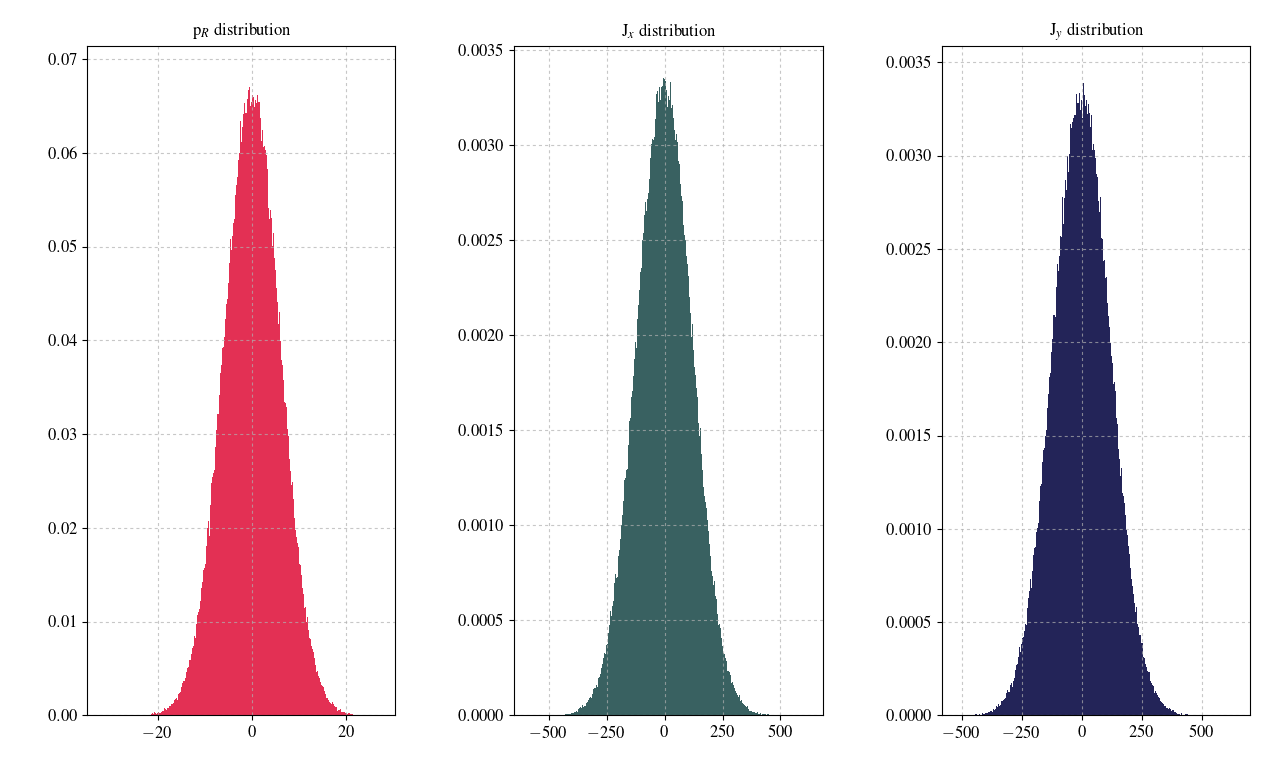
\includegraphics[width=\textwidth]{../pictures/diatomicsDistributions.png}
		\caption{Распределения переменных $p_R$, $J_x$, $J_y$ для двух атомов с массами $m_{Ar}$ и $m_{CO_2}$ при $T = 300 K$, 500.000 точек.}
\end{figure}

\begin{lstlisting}
#include <iostream>
#include <random>

using namespace std;

// boltzamnn constant 
const double BOLTZCONST = 1.38064e-23;
// dalton to kg 
const double DALTON = 1.660539e-27;
// atomic length unit to m 
const double ALU = 5.29177e-11;

// reduced mass of ar and co2 = m(ar) * m(co2) / (m(ar) + m(co2)) in kg
const double MU = 20.952 * DALTON;

// planck constant 
const double HBAR = 1.0545718e-34;

const double temperature = 300;

// distance between atoms 
const double RDIST = 20.0;

// a Mersenne Twister pseudo-random generator of 32-bit numbers with a state size of 19937 bits
static thread_local mt19937 generator;
 
double nextGaussian( const double &mean, const double &sigma )
{
    normal_distribution<double> d( mean, sigma );
    return d( generator ); 
} 

int main( int argc, char* argv[] )
{
	int n = atoi( argv[1] );

	for ( int i = 0; i < n; i++ )
	{
		double jx = nextGaussian( 0, RDIST * ALU * sqrt(BOLTZCONST * temperature * MU )) / HBAR;
		double jy = nextGaussian( 0, RDIST * ALU * sqrt(BOLTZCONST * temperature * MU )) / HBAR;
		double pR = nextGaussian( 0, sqrt(BOLTZCONST * temperature * MU)) / HBAR * ALU;

		cout << jx << "  " << jy << "  " << pR << endl;
	}

	return 0;
}
\end{lstlisting}

Пример программы на С++ для генерации значений $J_x$, $J_y$ и $p_R$ по точным распределениям \eqref{distr_exact}.


\subsection{Равномерно распределенные матрицы поворота}

Следующий алгоритм к получению равномерно распределенных матриц поворота состоит из двух шагов:
\begin{enumerate}
\item равномерно распределенный поворот вокруг оси $OZ$
\item поворот, приводящий к равномерному на сфере положению северного полюса
\end{enumerate} 

Первый шаг осуществить легко; пусть случайная величина $x_1$ равномерно распределена на отрезке $[0, 1]$, тогда матрица $R$ осуществляет равномерно распределенный поворот вокруг оси $OZ$ 
\begin{gather}
R =
\begin{bmatrix}
\cos \lb 2 \pi x_1 \rb & \sin \lb 2 \pi x_1 \rb & 0 \\
- \sin \lb 2 \pi x_1 \rb & \cos \lb 2 \pi x_1 \rb & 0 \\
0 & 0 & 1
\end{bmatrix} \label{rmatrix} 
\end{gather}

Второй шаг может быть выполнен при помощи \textit{преобразования Хаусхолдера} (Householder transform). Точка $z = (0, 0, 1)$  может быть перенесена в любую точку сферу при помощи отражения относительно плоскости, перпендикулярной вектору $\overline{zp}$ и проходящей через центр координат $O$. Такое отражение описывается \textit{Хаусхолдеровской матрицей}
\begin{gather}
		H = 1 - 2 v v^\top, \notag
\end{gather}
где $v$ -- единичный вектор, параллельный $\overline{zp}$. Взяв комбинацию хаусхолдеровского отражения и инверсии мы получим поворот, т.к. детерминант такого преобразования будет равен $\det(\cdot) = + 1$ (матрица преобразования будет равна $-H$). Таким образом, искомоая матрица поворота равна
\begin{gather}
		M = - HR \notag
\end{gather}

Матрица поворота $M$ будет равномерно распределена внутри $SO(3)$, если $H$ равномерно преобразует Северный полюс в любую точку на сфере, а $R$ описывает равномерный поворот вокруг $OZ$. Оператор $H$ будет удовлевторять поставленному условию, если мы возьмем
\begin{gather}
		v = 
		\begin{bmatrix}
				\cos \lb 2 \pi x_2 \rb \sqrt{x_3} \\
				\sin \lb 2 \pi x_2 \rb \sqrt{x_3} \\
				\sqrt{1 - x_3}
		\end{bmatrix}, \notag
\end{gather}
где $x_2$, $x_3$ -- равномерно распределены на $[0, 1]$. В таком случае матрица $H$ принимает следующий вид
\begin{gather}
		H = 1 - 2 v v^\top = 
		\begin{bmatrix}
			1 - 2 \cos^2 \lb 2 \pi x_2 \rb x_3 & -2 \sin \lb 2 \pi x_2 \rb \cos \lb 2 \pi x_2 \rb x_3 & - 2 \cos \lb 2 \pi x_2 \rb \sqrt{x_3 \lb 1 - x_3 \rb} \\
			- 2 \sin \lb 2 \pi x_2 \rb \cos \lb 2 \pi x_2 \rb x_3 & 1 - 2 \sin^2 \lb 2 \pi x_2 \rb x_3 & -2 \sin \lb 2 \pi x_2 \rb \sqrt{x_3 \lb 1 - x__3 \rb} \\
		- 2 \cos \lb 2 \pi x_2 \rb \sqrt{x_3 \lb 1 - x_3 \rb} & - 2 \sin \lb 2 \pi x_2 \rb \sqrt{x_3 \lb 1 - x_3 \rb} & 2 x_3 - 1
		\end{bmatrix} \notag
\end{gather}

Действие $H$ на вектор $z$ приводит к вектору $p$, компоненты которого равны
\begin{gather}
		 p = H z = \lb 1 - 2 v v^\top \rb \begin{bmatrix} 0 \\ 0 \\ 1 \end{bmatrix} =
		\begin{bmatrix}
				- 2 \cos \lb 2 \pi x_2 \rb \sqrt{x_3 \lb 1 - x_3 \rb} \\
				- 2 \sin \lb 2 \pi x_2 \rb \sqrt{x_3 \lb 1 - x_3 \rb} \\
				2 x_3 - 1
		\end{bmatrix} \notag
\end{gather}

Заметим, что если положить $\sin \phi = - 2 \sqrt{x_3 \lb 1 - x_3 \rb}$, то тогда $\cos \phi = 2 x_3 - 1$. Действительно,
\begin{gather}
	\sin^2 \phi + \cos^2 \phi = \left[ - 2 \sqrt{x_3 \lb 1 - x_3 \rb} \right]^2 + \left[ 2 x_3 - 1 \right]^2 = 1 \notag
\end{gather}

То есть, вектор $p$ может быть представлен в следующей форме
\begin{gather}
	p = 
	\begin{bmatrix}
		\cos \lb 2 \pi x_2 \rb \sin \varphi \\
		\sin \lb 2 \pi x_2 \rb \sin \varphi \\
		\cos \varphi
	\end{bmatrix} = 
	\begin{bmatrix}
		\cos \lb 2 \pi x_2 \rb \sqrt{z} \\
		\sin \lb 2 \pi x_2 \rb \sqrt{z} \\
		\sqrt{1 - z}
	\end{bmatrix}. \notag
\end{gather}
Следовательно $p$ равномерно распределен на сфере, т.к. азимутальный угол и косинус полярного угла $\cos \varphi = 2 x_3 - 1$ распределены равномерно на $[-1, 1]$. Для упрощения компонент вектора переобозначим $\sqrt{z} = \sqrt{x_3 \lb 1 - x_3 \rb}, \sqrt{1 - z} = 2 x_3 - 1 $. Итак, схема алгоритма представлена ниже.

\begin{algorithm}[H]
\begin{algorithmic}[1]
\caption{Generation of random rotation matrices [3]} \label{randrot}
\State $x_1$, $x_2$, $x_3$ $\gets$ 3 random variables uniformly distributed over $[0, 1]$  
\State Pick a rotation about the pole: $\theta \gets 2 \pi x_1$  
\State Pick a direction to deflect the pole: $\phi \gets 2 \pi x_2$
\State Pick the amount of pole deflection: $z \gets x_3$.
\State Construct a vector to perform the reflection: 
v = 
\begin{bmatrix}
	\cos \phi \sqrt{z} \\
	\sin \phi \sqrt{z} \\
	\sqrt{1 - z}
\end{bmatrix}
\State Construct the rotation matrix by combining two simple rotations: first rotate about the $Z$-axis, then rotate the $Z$-axis to a random orientation: 
$
M \gets \lb 2 v v^\top - 1 \rb
\begin{bmatrix}
		\cos \theta & \sin \theta & 0 \\
		-\sin \theta & \cos \theta & 0 \\
		0 & 0 & 1
\end{bmatrix}
$.
\end{algorithmic}
\end{algorithm}

\begin{lstlisting}
#include <iostream>
#include <random>
#include <Eigen/Dense>

using namespace std;
using namespace Eigen;

//a Mersenne Twister pseudo−random generator of 32−bit numbers with a state size of 19937 bits 
random_device rd;
mt19937 eng( rd() );
uniform_real_distribution<double> distr( 0.0, 1.0);

void rotationMatrix( Matrix3d &m )
{
	double theta = 2 * M_PI * distr( eng ); // a rotation about the pole
	double phi = 2 * M_PI * distr( eng ); // a direction to deflect the pole 
	double z = distr( eng ); // the amount of pole deflection	 
	double sz = sqrt( z );

	// a vector to perform the reflection
	Vector3d v ( cos(phi) * sz, sin(phi) * sz, sqrt(1 - z) );
	// the Householder matrix
	Matrix3d s = 2 * v * v.transpose() - Matrix<double, 3, 3>::Identity();

	Matrix3d r;
   	r << cos(theta), sin(theta), 0,
		-sin(theta), cos(theta), 0,
		0, 0, 1;
	
	m = s * r;
}

int main( int argc, char* argv[] )
{
	int n = atoi( argv[1] );
	
	// initial vector
	Vector3d v ( 0.0, 0.0, 1.0 );
	// resulting vector
	Vector3d r;

	for ( int i = 0; i < n; i++ )
	{
		// filling rotation matrix
    	Matrix3d m;
    	rotationMatrix( m );

		// performing a random rotation of OZ-vector
		r = m * v;
		
		// displaying the components of resulting vector
		cout << r(0) << " " << r(1) << " " << r(2) << endl;
	}

    return 0;
}
\end{lstlisting}

Пример программы на C++ с применением библиотеки линейной алгебры $Eigen$. Программа принимает на вход количество рассчитываемых векторов $n$. Внутри главного цикла генерируется по описанному алгоритму случайная матрица поворота и применяется для поворота вектора $v = \left[ 0, 0, 1 \right]$. На выходе получаем $n$ равномерно распределенных на сфере векторов.

\begin{figure}[ht!]
	\begin{center}
		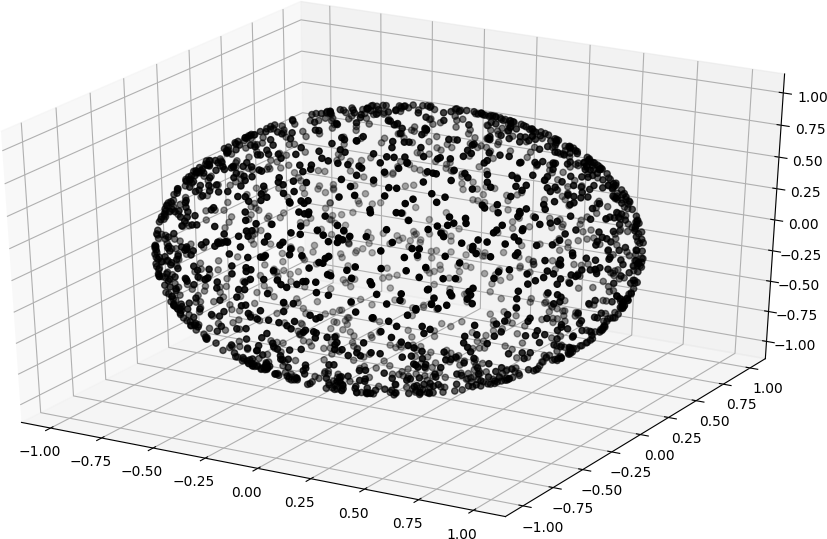
\includegraphics[width=0.5\textwidth]{../pictures/sphere_dots.png}
	\end{center}
		\caption{Пример равномерно распределенных на сфере точек, полученных в результате приведенной выше программы. 2000 точек.}
\end{figure}




\subsection{MCMC-sampling}

Как известно, в каноническом ансамбле плотность вероятности в фазовом пространстве определяется гамильтонианом [4]
\begin{gather}
	\rho \lb \mf{q}, \mf{p}, \mf{J} \rb \propto \exp \lb - \frac{H \lb \mf{q}, \mf{p}, \mf{J} \rb}{k T} \rb  \notag
\end{gather}
Таким образом, задача получения распределений $\mf{q}, \mf{p}, \mf{J}$ может быть рассмотрена как задача сэмплинга точек в фазовом пространстве согласно известной плотности вероятности. Попытаемся решить эту задачу при помощи метода \textit{Markov Chain Monte Carlo} (MCMC); суть метода заключается в построении Марковской цепи в фазовом пространстве, стационарное распределение которой совпадает с целевым распределением. Фактически, в нашем случае мы будем рассматривать не полное фазовое пространство, а его сечение -- $R = const$. \par
Предположим мы генерируем последовательность случайных величин, $\left\{ X_0, X_1, X_2, \dots \right\}$, так что в каждый момент $t \geq 0$ следующее состояние $X_{t + 1}$ выбирается исходя из распределения $P \lb X_{t+1} | X_t \rb$, которое зависит от текущего состояния $X_t$, но не от предыдущего набора состояний $\left\{ X_0, X_1, X_2 ... X_{t - 1} \right\}$. То есть, состояние $X_{t + 1}$ определяется исключительно предыдущим $X_t$. Такая последовательность состояний называется \textit{цепью Маркова}. \par
Перейдем к рассмотрению алгоритма Метрополиса-Гастингса, представляющего собой один из простейших алгоритмов для построения Марковской цепи с заданным стационарным распределением $\pi \lb \cdot \rb$.

\begin{algorithm}
\begin{algorithmic}[2]
		\caption{Scheme of Metropolis-Hastings algorithm from [1]}\label{metropolis}
\State Initialize $x^{(0)} \sim q(x)$
\State \textbf{for} iteration $i = 1, 2, \dots$ \textbf{do}
\State \quad Propose: $x^{cand} \sim q \lb x^{(i)} | x^{(i-1)} \rb$
\State \quad Acceptance probability:
\State \qquad $\alpha \lb x^{cand} | x^{(i-1)} \rb = \min \left\{ 1, \frac{q \lb x^{(i-1)} | x^{cand} \rb \pi \lb x^{(cand)} \rb }{ q \lb x^{cand} | x^{(i-1)} \rb \pi \lb x^{(i-1)} \rb} \right\}$
\State \quad $u \sim$ Uniform(u; 0, 1)
\State \quad \textbf{if} $u < \alpha$ \textbf{then}
\State \qquad Accept the proposal: $x^{(i)} \gets x^{cand}$
\State \quad \textbf{else}
\State \qquad Reject the proposal: $X^{(i)} \gets x^{(i-1)}$
\State \quad \textbf{end if}
\State \textbf{end for}
\end{algorithmic}
\end{algorithm}

Первым шагом алгоритма является выбор стартовой точки цепи, определенных методик, насколько я понимаю, здесь нет; в целом важно не задавать ее в какой-то "нефизичной" области фазового пространства (в той, в которой очень маловероятно застать рассматриваемую систему). Следующий за ним главный цикл алгоритма состоит из трех частей: (1) получить следующую точку ("кандидата") $x^{cand}$ исходя из вспомогательного распределения $q \lb x^{(i)} | x^{(i-1)} \rb$; (2) рассчитать вероятность перехода в новую точку $\alpha \lb x^{cand} | x^{(i-1)} \rb$, основываясь на распределении $q$ и функции распределения $\pi$; (3) принять новую точку с вероятностью $\alpha$. \par
Обратим внимание на то, что точка, полученная исходя из вспомогательного распределения $q(\cdot)$, принимается не всегда, а лишь с вероятностью $\alpha \lb \cdot \rb$. Рассматривают вспомогательные распределения двух классов -- симметричные и асимметричные. Симметричным называется распределение, удовлетворяющее следующему соотношению
\begin{gather}
		q \lb x^{(i)} | x^{(i-1)} \rb = q \lb x^{(i-1)} | x^{(i)} \rb \notag
\end{gather}
К часто используемым симметричным распределениям относятся гауссово и равномерное распределения. В качестве примера рассмотрим вспомогательное распределение Гауссса: 
\begin{gather}
		x^{cand} = x^{(i-1)} + Normal(0, \sigma) \notag
\end{gather}

Понятно, что $Normal( x^{cand} - x^{(i-1)}; 0, \sigma ) = Normal( x^{(i-1)} - x^{cand}; 0, \sigma)$, то есть Гауссово распределение в действительности задает симметричное вспомогательное распределение. Среднеквадратичное отклонение $\sigma$ является параметром модели. Значение этого параметра будет определять динамику Марковской цепи в рассматриваемом пространстве. \par
В случае симметричных вспомогательных распределений выражение для вероятности выбора новой точки $\alpha(\cdot)$ существенно упрощается:
\begin{gather}
		\alpha \lb x^{cand} | x^{(i-1)} \rb = \min \left\{ 1, \frac{\pi \lb x^{cand} \rb}{\pi \lb x^{(i - 1)} \rb} \right\} \notag 
\end{gather}

Заметим, что если плотность вероятности ( точнее говоря, величина, пропорциональная плотности вероятности ) в новой точке $\pi \lb x^{cand} \rb$ больше, чем плотность вероятности в текущей $\pi \lb x^{\lb i - 1 \rb} \rb$, то их отношение будет больше $1$, а значит вероятность перехода в новую точку будет равна 1: $\alpha \lb x^{cand} | x^{(i - 1)} \rb = 1$. Другими словами, если новая точка выбрана таким образом, что плотность вероятности в ней больше, чем в текущей, то в нее осуществляется переход. Устройство алгоритма таково, что Марковская цепь "склонна" посещать те точки пространства, в которых моделируемая плотность вероятности выше. Однако, если новая точка была выбрана таким образом, что плотность вероятности в ней меньше, чем в текущей, то тогда вероятность перейти в нее будет определяться отношением плотностей вероятности:
\begin{gather}
		\alpha \lb x^{cand} | x^{(i - 1)} \rb = \frac{\pi \lb x^{cand} \rb}{\pi \lb x^{(i - 1)} \rb} \notag
\end{gather}

То есть, если вероятность в новой точке будет мала по сравнению с текущей, то и переход в нее будет маловероятен. Заметим, что при подсчете вероятности нам нужно знать лишь отношение плотностей вероятности, а не ее абсолютное значение; поэтому в качестве $\pi \lb \cdot \rb$ можно брать не плотность вероятности, а величину ей пропорциональную. \par
Вид вероятности перехода в новую точку из текущей определяется \textit{условием детального баланса} [2]. Последнее гарантирует, что полученная Марковская цепь в действительности будет удовлетворять заданной плотности вероятности.



\subsection{Parallel Metropolis-Hastings}

...


\section{Начальные распределения для CO$_2-$Ar}
\subsection{Точные формулы для распределений}

Из классической механики известно, что при отделении центра масс в системе <<атом + линейная молекула>> образуются две эффективные частицы, где первая частица движется на расстоянии $l$ и имеет массу $\mu_1=\frac{m_1 m_2}{m_1+m_2}$, а вторая, с массой $\mu_2 = \frac{(m_1+m_2)m_3}{m_1+m_2+m_3}$ движется на расстоянии $R$, где $R$ -- расстояние между центром масс линейной молекулы и атомом, $l$ -- длина линейной молекулы.\\
\\
Тогда для связи векторов в ЛСК и МСК у нас получатся слеующие выражения:
\begin{equation}
\label{eq:relation_mol_lab}
\begin{array}{c}
\bbS \, \dot{\mf{r}}_1 = 
 \Bigg\{ \left( \begin{matrix}
l \cos (\Theta )\dot \Theta\\ 
0\\
-l \sin (\Theta) \dot \Theta
\end{matrix}  \right) + 
\left( \begin{matrix}
l\Omega_y \cos (\Theta) \\ 
-l\Omega_x \cos(\Theta) + l\Omega_z \sin(\Theta)\\
-l\Omega_y \sin(\Theta)
\end{matrix}  \right) \Bigg\}\\
\bbS \, \dot{\mf r}_2 =  \Bigg\{ \left( \begin{matrix}
0\\ 
0\\
\dot R
\end{matrix}  \right) + 
\left( \begin{matrix}
\Omega_y R\\ 
-\Omega_x R\\
0
\end{matrix}  \right) \Bigg\}
\end{array}
\end{equation}
причем $\bbS$ -- ортогональная матрица поворота, например, матрица углов Эйлера. 
Для упрощения дальнейших выкладок тильдой пометим компоненты векторов, получающиеся при действии матрицы $\mathbb{S}$ на вектора скорости в лабораторной системе координат.

\begin{equation}
\label{eq:r_tilde}
\begin{array}{c}
\mathbb{S} \, \dot{\mf{r}}_1 = \bbS \left(\begin{matrix}
\dot{x}_1\\
\dot{y}_1\\
\dot{z}_1
\end{matrix}\right)  =
\left(\begin{matrix}
S_{11}\dot{x}_1 + S_{12}\dot{y}_1 + S_{13}\dot{z}_1 \\
S_{21}\dot{x}_1 + S_{22}\dot{y}_1 + S_{23}\dot{z}_1\\
S_{31}\dot{x}_1 + S_{32}\dot{y}_1 + S_{33}\dot{z}_1
\end{matrix}\right)
=  \left(\begin{matrix}
\tilde{r}_{11}\\
\tilde{r}_{12}\\
\tilde{r}_{13}
\end{matrix}\right)
\\
\bbS \, \dot{\mf{r}}_2 = \mathbb{S}\left(\begin{matrix}
\dot{x}_2\\
\dot{y}_2\\
\dot{z}_2
\end{matrix}\right)  =
\left(\begin{matrix}
S_{11}\dot{x}_2 + S_{12}\dot{y}_2 + S_{13}\dot{z}_2 \\
S_{21}\dot{x}_2 + S_{22}\dot{y}_2 + S_{23}\dot{z}_2\\
S_{31}\dot{x}_2 + S_{32}\dot{y}_2 + S_{33}\dot{z}_2
\end{matrix}\right)= \left(\begin{matrix}
\tilde{r}_{21}\\
\tilde{r}_{22}\\
\tilde{r}_{23}
\end{matrix}\right) 
\end{array}
\end{equation}

\begin{equation}
\mL = \frac{\mu_1}{2}\dot{\mf{r}}_1^2 + \frac{\mu_2}{2}\dot{\mf{r}}_2^2 - U(R,\Theta)
\end{equation}

Запишем (\ref{eq:relation_mol_lab}) в качестве системы уравнений, с учетом (\ref{eq:r_tilde}).

\begin{equation}
\label{eq:system}
\begin{cases}
\tilde{r}_{11} = l \dot{\Theta} \cos \Theta  + l\Omega_y \cos \Theta \\
\tilde{r}_{12} = -l\Omega_x \cos \Theta + l\Omega_z \sin \Theta \\
\tilde{r}_{13} = -l \dot{\Theta} \sin \Theta - l \Omega_y \sin \Theta \\
\tilde{r}_{21} = \Omega_y R\\
\tilde{r}_{22} = -\Omega_x R\\
\tilde{r}_{21} = \dot R
\end{cases}
\end{equation}
Предполагая, что в (\ref{eq:system}) 1-е и 3-е уравнения эквивалентны (в конце документа рассмотрен случай отсутствия этого предположения), найдем выражения для скоростей в МСК, решая данную систему линейных уравнений:
\begin{gather}
\left\{
\begin{aligned}
\dot R &= \tilde{r}_{23}\\
\dot \Theta &= -\frac{1}{l\sin \Theta} \lb \tilde{r}_{13}+\frac{1}{R} \tilde{r}_{21} \, l \sin\Theta  \rb \\
\Omega_x &= -\frac{1}{R}\tilde{r}_{22} \\
\Omega_y &= \frac{1}{R} \tilde{r}_{21} \\
\Omega_z &= \frac{1}{\sin \Theta} \lb \tilde{r}_{12}- \frac{1}{R} \tilde{r}_{22}l\cos \Theta \rb
\end{aligned}
\right.
\end{gather}

Мы не будем приводить здесь вывод, однако несложно показать, что гамильтоновы переменные связаны с лагранжевыми переменными для рассматриваемой системы следующим образом:

\begin{gather}
\left\{
\begin{aligned}
p_R &= \mu_2\dot R\\
p_{\Theta} &= \Omega_yl^2 \mu_1 + l^2 \mu_1 \dot \Theta \\
J_x &= -\mu_1 l^2 \Omega_z \sin \Theta \cos \Theta + \Omega_x \lb \mu_1 l^2 \cos^2 \Theta + \mu_2 R^2 \rb \\
J_y &= \mu_1 l^2 \dot \Theta + \Omega_y \lb \mu_2 R^2 + \mu_1 l^2 \rb \\
J_z &= -l^2 \mu_1 \sin \Theta \lb \Omega_x \cos\Theta - \Omega_z \sin\Theta \rb
\end{aligned}
\right.
\end{gather}

Теперь подставим выражения для скоростей в выражения для импульсов.
\begin{gather}
\left\{
\begin{aligned}
p_R &= \mu_2 \tilde{r}_{23}\\
p_{\Theta} &= -\frac{\mu_1 l}{\sin\Theta}\tilde{r}_{13} \\
J_x &= -\mu_2 R \tilde{r}_{22} - \mu_1 l \tilde{r}_{12} \cos \Theta \\
J_y &= \mu_2 R \tilde{r}_{21} - \frac{\mu_1 l}{\sin \Theta}\tilde{r}_{13} \\
J_z &= \mu_1 l\tilde{r}_{12} \sin \Theta
\end{aligned}
\right.
\end{gather}

Рассмотрим вопрос о распределении компонент векторов $\dot{\mf{r}}_1$ и $\dot{\mf{r}}_2$. 
Представим вектор $\dot{\mf{r}}_1$ в лабораторной системе в сферических координатах $\begin{bmatrix} l, & \phi, & \theta \end{bmatrix}$: 
\begin{gather}
\dot{\mf{r}}_1 = \frac{d}{dt}
\begin{bmatrix}
l \sin \theta \cos \phi\\
l \sin \theta \sin \phi\\
l\cos \theta
\end{bmatrix}
=
\begin{bmatrix} 
l \dot{\theta} \cos\theta \cos\phi  - l \dot{\phi} \cos\theta \sin\phi \\ 
l \dot{\theta} \cos\theta \sin\phi + l \dot{\phi} \sin\theta \cos\phi \\ 
 -l \dot{\theta} \sin \theta 
\end{bmatrix} \notag 
\end{gather}

Нетрудно видеть, что вектора $\dot{\boldsymbol{\theta}}$ и $\dot{\boldsymbol{\phi}} \sin \phi$ направлены перпендикулярно оси вращения линейной молекулы, а значит, являются угловыми скоростями вращения линейной молекулы, поэтому распределены как $\mathcal{N}(0,kT/I)$, где $I$ -- момент инерции линейной молекулы. \par
Ради интереса отметим, что будет, если в системе (\ref{eq:system}) не считать 1-е и 3-е уравнения эквивалентными. Для этого умножим первое уравнение на $\sin\Theta$, а второе на $\cos\Theta$, после этого получим
\[
\sin\Theta \: \tilde{r}_{11} + \cos\Theta \: \tilde{r}_{13} = 0
\]
\[
\cot\Theta = -\frac{\tilde{r}_{13}}{\tilde{r}_{11}}
\]
Если $\tilde{r}_{11}$ и $\tilde{r}_{13}$ нормально распределенные случайные величины, то $\cot\Theta$ имеет распределение Коши. \par
Заметим, что алгоритм MH для получения начальных условий может быть применен как только имеется процедура расчета гамильтониана в произвольной точке фазового пространства. Распределения для $\Theta$, $p_R$, $p_T$, $J_x$, $J_y$, $J_z$, полученные по точным формулам и при помощи алгоритма MH, представлены на рис. $\ref{fig:co2ar_comparison}$. Распределение угла $\Theta$ (как угла между двумя равномерно на сфере распределенными векторами) имеет плотность вероятности $f(x) = \displaystyle \frac{1}{2} \sin x$ (на рисунке представлено пунктирной линией), это показано в приложении \ref{app4}.


\begin{figure}[!ht]
	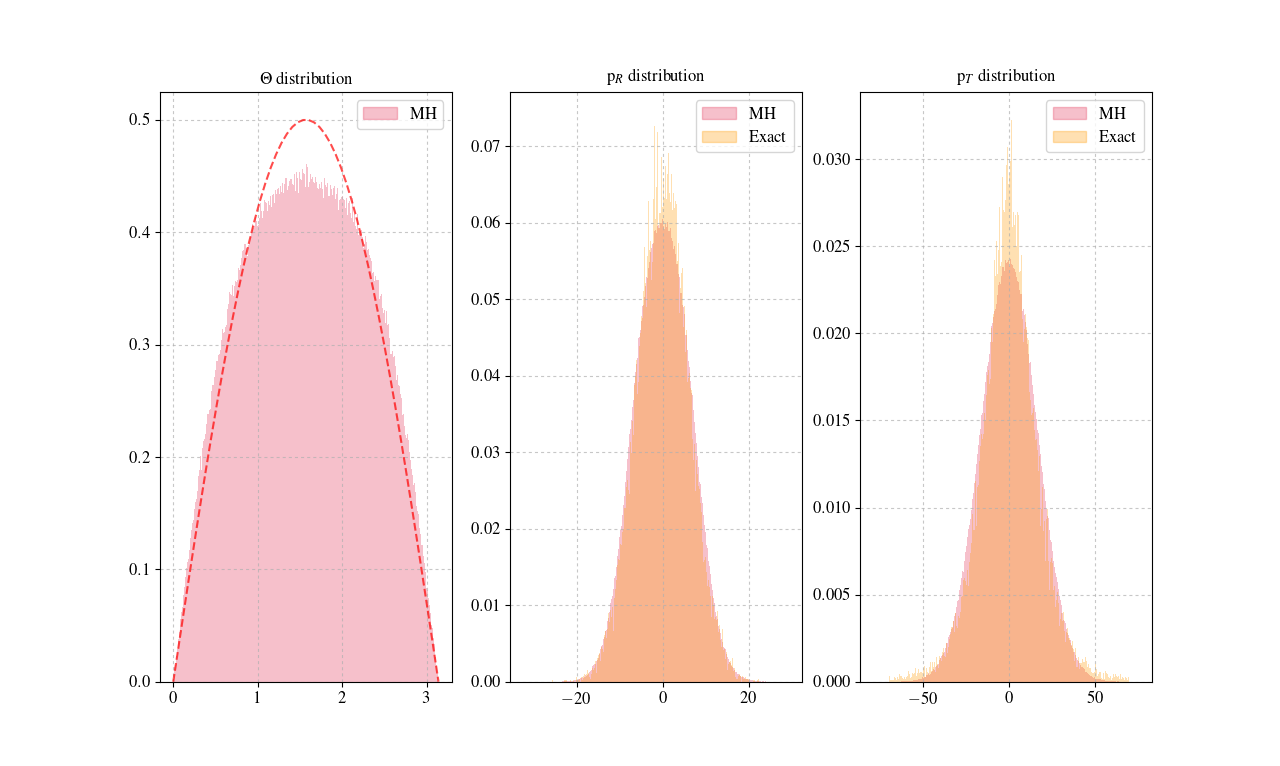
\includegraphics[width=\textwidth]{../pictures/co2arDistributions1.png}
	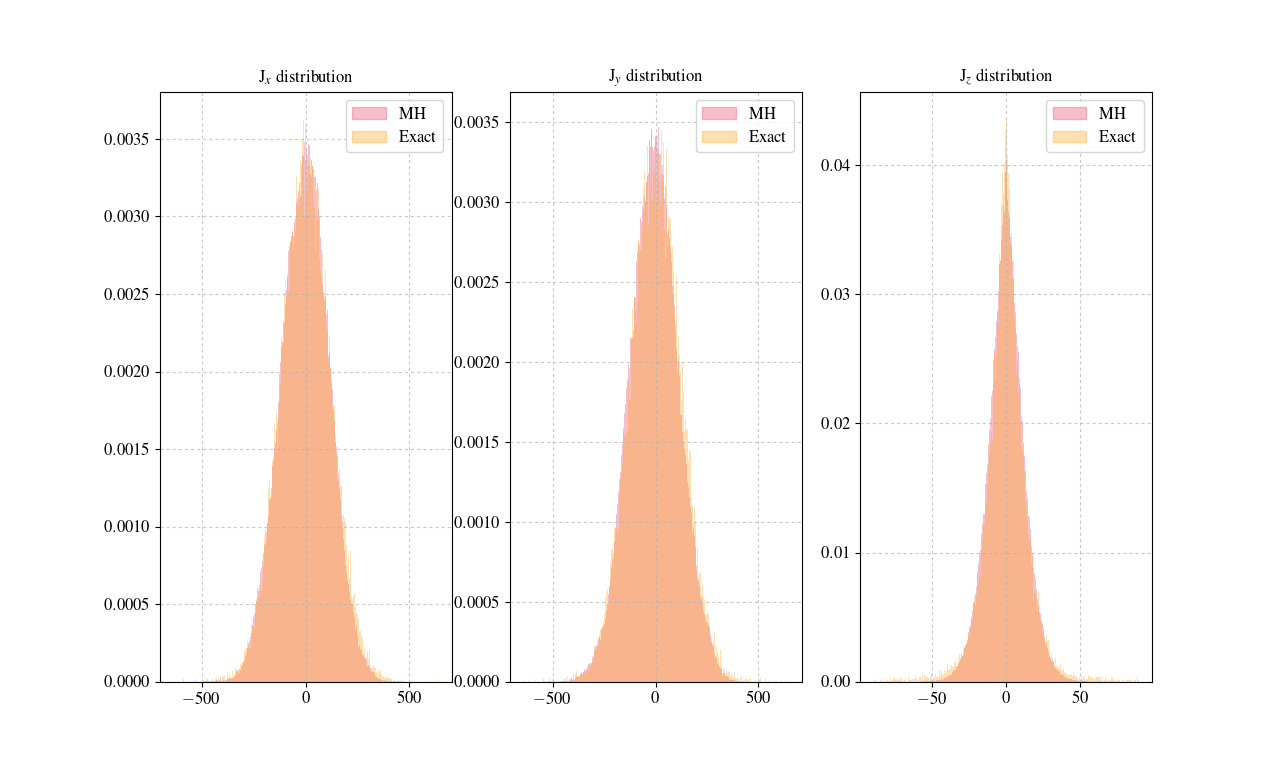
\includegraphics[width=\textwidth]{../pictures/co2arDistributions2.png}
	\caption{Распределения переменных $\Theta$, $p_R$, $p_T$ (\textbf{первый ряд}), $J_x$, $J_y$, $J_z$ (\textbf{второй ряд}) для CO$_2-$Ar при $T = 300 K$, полученные методом $MH$ и по точным формулам, 500.000 точек, $R$ = 20 бор.}
	\label{fig:co2ar_comparison}
\end{figure}




\section{Распределения для связанных состояний CO$_2-$Ar}


Для нахождения распределений гамильтоновых переменных в связанных состояниях CO$_2-$Ar сформируем Марковскую цепь в подпространстве $H < 0$ фазового пространства $\Gamma$. Генерацию точек Марковской цепи также осуществим методом MH с некоторой модификацией.

\begin{algorithm}[!h]
\begin{algorithmic}[1]
		\caption{Scheme of modified Metropolis-Hastings algorithm} \label{bound}
\State Initialize $x^{(0)} \sim q(x)$
\State \textbf{for} iteration $i = 1, 2, \dots$ \textbf{do}
\State \quad Propose: $x^{cand} \sim q \lb x^{(i)} | x^{(i-1)} \rb$
\State \quad Calculate: $E^{cand} = H \lb x^{cand} \rb$ 
\State \quad \textbf{if} $E^{cand} > 0$ \textbf{then}
\State \qquad Reject the proposal: $x^{(i)} \gets x^{(i - 1)}$
\State \quad \textbf{else}
\State \qquad \textbf{continue}
\State \quad \textbf{end if}
\State \quad Acceptance probability:
\State \qquad $\alpha \lb x^{cand} | x^{(i-1)} \rb = \min \left\{ 1, \frac{q \lb x^{(i-1)} | x^{cand} \rb \pi \lb x^{(cand)} \rb }{ q \lb x^{cand} | x^{(i-1)} \rb \pi \lb x^{(i-1)} \rb} \right\}$
\State \quad $u \sim$ Uniform(u; 0, 1)
\State \quad \textbf{if} $u < \alpha$ \textbf{then}
\State \qquad Accept the proposal: $x^{(i)} \gets x^{cand}$
\State \quad \textbf{else}
\State \qquad Reject the proposal: $x^{(i)} \gets x^{(i-1)}$
\State \quad \textbf{end if}
\State \textbf{end for}
\end{algorithmic}
\end{algorithm}

Модификация алгоритма описана на строчках 4-9. После выбора кандидата -- возможной следующей возможной точки цепи -- вычисляем значение гамильтониана $H$ в выбранной точке фазового пространства. Если энергия $E^{cand}$ больше 0, то это состояние не является связанным, и оно отвергается. Если же энергия $E^{cand} < 0$, то к нему применяется стандартная процедура алгоритма MH. Таким образом Марковская цепь разворачивается в подпространстве фазового пространства $H < 0$. Полученные распределения представлены на рис. \ref{fig:bound}. Заметим, что распределение по $\Theta$ обладает заметной анизотропией (пунтирной линией на графике показано распределение для несвязанных состояний).

\begin{figure}[!ht]
	\vspace*{-0.5cm}
	\newcommand{h}{5cm}
	\centering 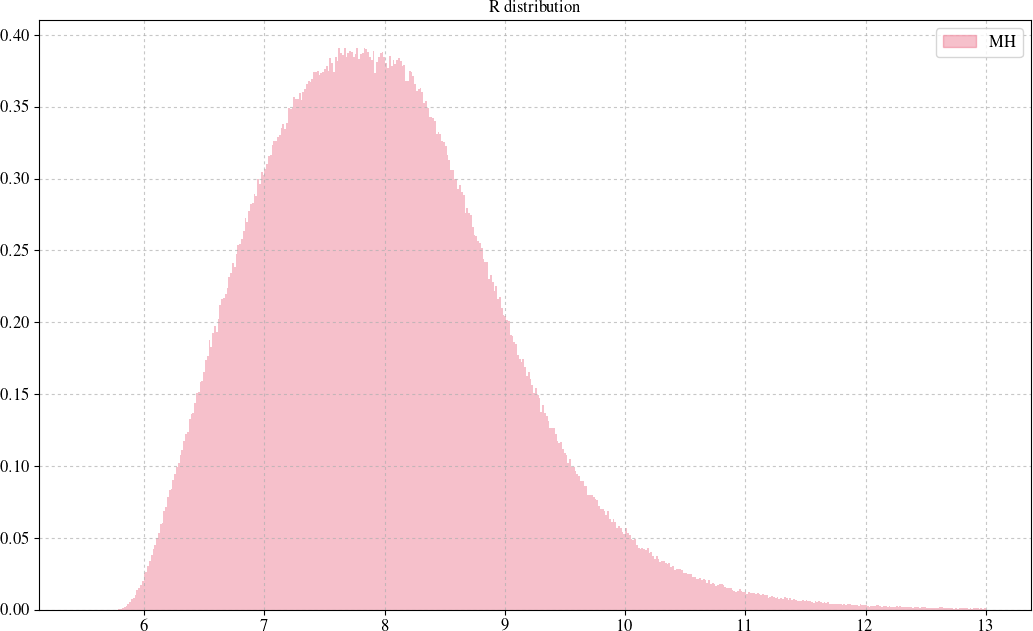
\includegraphics[width=0.5\textwidth, height=5cm]{../pictures/r_bound_distribution.png} \\ 
	\vspace{0.2cm}
	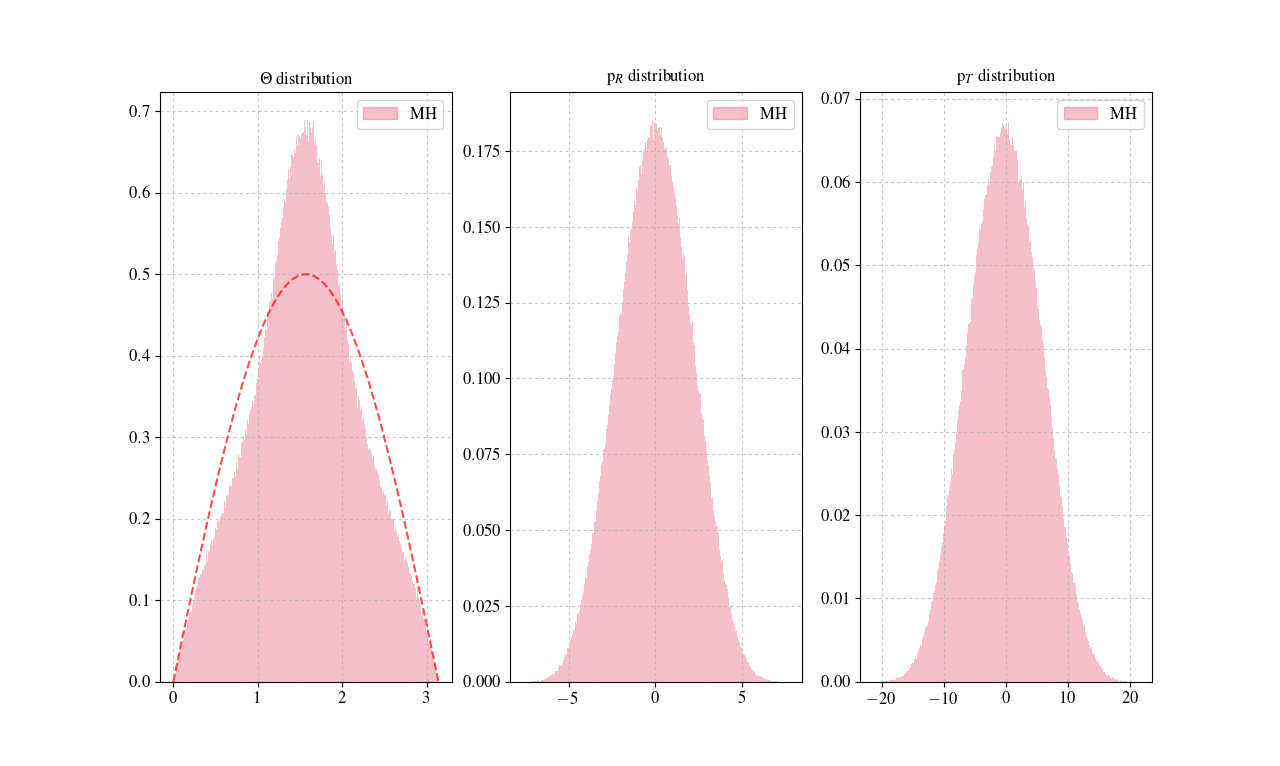
\includegraphics[width=0.8\textwidth, height=6cm]{../pictures/theta_bound_distribution.png} \\
	\vspace{0.2cm}
	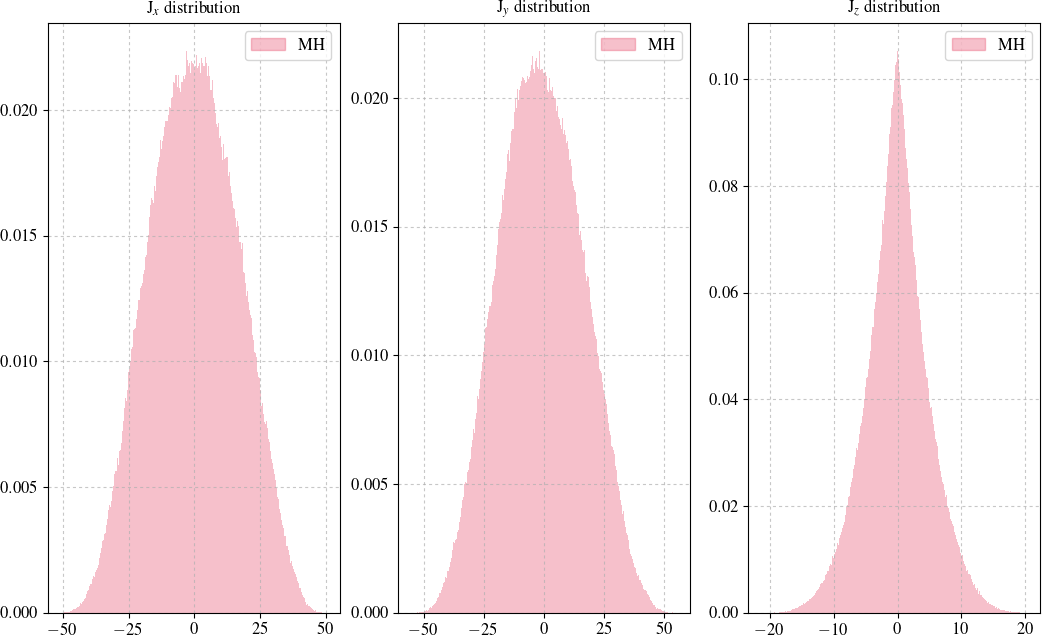
\includegraphics[width=0.7\textwidth, height=6cm]{../pictures/j_bound_distribution.png} 
\caption{Распределения переменных $R$, (\textbf{первый ряд}), $\Theta$, $p_R$, $p_T$ (\textbf{второй ряд}), $J_x$, $J_y$, $J_z$ (\textbf{третий ряд}) для связанных состояний CO$_2-$Ar при $T = 300 K$, полученные модифицированным методом MH, 2.000.000 точек}
	\label{fig:bound}
\end{figure}



\section{Веса траекторий при расчете спектра поглощения}

Рассмотрим случайный вектор начальных условий $\boldsymbol{\xi} = {(\Theta, p_R, p_{\Theta},J_X, J_Y, J_Z)}$. Очевидно, что отношение частот появления начальных условий, описываемых вектором $\boldsymbol{\xi}$ при двух разных температурах $T_1$ и $T_2$ будет определяться соотношением:

\begin{gather}
\lambda = \frac{P(\boldsymbol{\xi}, T_1)}{P(\boldsymbol{\xi}, T_2)} = \frac{\exp \lb - H \lb \boldsymbol{\xi} \rb / kT_1 \rb}{ \exp \lb -H \lb \boldsymbol{\xi} \rb / kT_2 \rb} \notag 
\end{gather}

Спектральная функция вычисляется по траекториям следующим образом:
\begin{gather}
J(\omega) = \frac{1}{N} \sum_{i=1}^{N} \hat{A} \lb \mu_i(t) \rb \label{eq:J_traj} 
\end{gather}

где $N$ -- число траекторий, а $\hat A$ -- определенного вида операция, производимая для дипольного момента на каждой траектории (квадрат модуля преобразования Фурье). Тогда вполне очевидно, что для пересчета спектральной плотности на другую температуру мы должны домножить каждый член суммы в числителе (\ref{eq:J_traj}) на соответствующий коэффициент пересчета $\lambda_i$, не забыв учесть нормировку в знаменателе.
\begin{gather}
J(\omega, T_2) = \frac{\displaystyle \sum_{i = 1}^{N} \lambda_i \hat{A} \lb \mu_i(t) \rb}{\displaystyle \sum_{i = 1}^{N}(\lambda_i \cdot 1) \label{eq:J_traj_lambda}}
\end{gather}

Для наглядности продемонстируем вышесказанное на простом примере. Пусть есть две траектории, причем коэффициент $\lambda$ для первой оказался равен $0.5$, а для второй -- $2$
\begin{equation*}
\begin{aligned}
J(\omega, T_1) = \frac{\hat A(\mu_1(t))+\hat A(\mu_2(t))}{2} = \frac{2\hat A(\mu_1(t))+2\hat A(\mu_2(t))}{4} = \\
\frac{\hat A(\mu_1(t))+\hat A(\mu_1(t))+\hat A(\mu_2(t))+\hat A(\mu_2(t))}{4}
\end{aligned}
\end{equation*}
Теперь если для первой траектории коэффициент равен $0.5$, то это означает, что при температуре $T_2$ начальное условие, соответствующее данной траектории будет встречаться в 2 раза меньше, чем при температуре $T_1$, а это означает, что в сумме (\ref{eq:J_traj}) мы в 2 раза реже будем писать преобразование от первой траектории, то есть таких членов в сумме будет в два раза меньше. Аналогичные рассуждения применяются и для второй траектории. В итоге:
\begin{equation*}
J(\omega, T_2) = \frac{\hat A(\mu_1(t))+4\hat A(\mu_2(t))}{5} = \frac{0.5\hat A(\mu_1(t))+2\hat A(\mu_2(t))}{2.5}
\end{equation*}
что соответствует формуле (\ref{eq:J_traj_lambda}).



\newpage
\section{Литература}
\begin{enumerate}
	\item Yildirim I. Bayesian Inference: Metropolis-Hastings Sampling. MIT Online Library
	\item Gilks, W.R., Richardson, S., \& Spiegelhalter, D.J. (1996). \textit{Markov Chain Monte Carlo in Practice}. London: Chapman and Hall.
	\item  Kirk D. Graphics Gems III. III. 4. Fast random rotation matrices. 
	\item Н. А. Смирнова. Методы статистической термодинамики в физической химии. (гл. 4)

	\item Marsaglia G. (1972). "Choosing a Point from the Surface of a Sphere". \textit{Annals of Mathematical Statistics}. \textbf{42} (2): 645-645.
\end{enumerate}

\newpage

\titleformat{\section}{\large\bfseries}{\appendixname~\thesection .}{0.5em}{}

\begin{appendices}
\addtocontents{toc}{\setcounter{tocdepth}{-1}}

\section{Приложение А. Распределения в лабораторной системе координат} \label{app1}

Воспользуемся следующими двумя выводами из теории вероятностей:
\begin{enumerate}
\item Пусть случайная величина $\xi$ распределена с плотностью $f_\xi \left( x \right)$. Тогда случайная величина $\eta = a \xi + b$ распределена с плотностью
\begin{gather}
	f_\eta (x) = \frac{1}{|a|} f_\xi \lb \frac{x - b}{a} \rb \notag
\end{gather}
\item Если две \underline{независимые} случайные величины $X$ и $Y$ распределены с плотностями $X \sim f_1(x)$ и $Y \sim f_2(x)$ соответственно, то случайна величина $Z = X + Y$ распределена с плотностью
\begin{gather}
	g(z) = \int\limits_{-\infty}^{+\infty} f_1(x) f_2(z - x) dx \notag
\end{gather}
\end{enumerate}

Т.к. вектор $\mf{r} = \mf{r}_1 - \mf{r}_2$ равен разнице радиус-векторов двух атомов $\mf{r}_1$ и $\mf{r}_2$ в лабораторной системе координат соответственно, то $\dot{\mf{r}} = \dot{\mf{r}}_1 - \dot{\mf{r}}_2$. Используя п.1 и п.2 получим распределение для компонент $\mf{r}$:
\begin{gather}
\left\{
\begin{aligned}
		\dot{\mf{r}}_{1x} &\sim f_1(x) = \sqrt{ \frac{m_1}{2 \pi k T} } \exp \lb - \frac{m_1 x^2}{2 k T} \rb \\
		- \dot{\mf{r}}_{2x} &\sim f_2(x) = \sqrt{ \frac{m_2}{2 \pi k T} } \exp \lb - \frac{m_2 x^2}{2 k T} \rb 
\end{aligned} \notag \\
\dot{\mf{r}}_x \sim \int\limits_{-\infty}^{+\infty} f_1(x) f_2(z - x) dx = \frac{ \sqrt{m_1 m_2}}{2 \pi k T} \int\limits_{-\infty}^{+\infty} \exp \lb - \frac{m_1 x^2}{2 k T} \rb \exp \lb - \frac{m_2 \lb z - x \rb^2}{2 k T} \rb dx 
\right. \label{r_distr}
\end{gather}

Отдельно рассмотрим получившийся интеграл:
\begin{gather}
		\intty \exp \lb - \frac{m_1 x^2}{2 k T} - \frac{m_2 \lb z - x \rb^2}{2 k T} \rb dx = \intty \exp \lb \frac{- \lb m_1 + m_2 \rb x^2 - m_2 z^2 + 2 m_2 z x}{2 k T} \rb dx = \notag \\
		= \intty \exp \lb - \frac{\lb \sqrt{m_1 + m_2} x - \frac{m_2}{\sqrt{m_1 + m_2}} z \rb^2}{2 k T} \rb \exp \lb - \frac{m_2 z^2 - \frac{m_2^2}{m_1 + m_2} z^2 }{2 k T} \rb dx = \notag \\
		= \left[ y = \frac{ \sqrt{m_1 + m_2} x - \frac{m_2}{\sqrt{m_1 + m_2}} z}{ \sqrt{2 k T} } \right] = \sqrt{ \frac{2 k T}{m_ 1 + m_2} } \exp \lb - \frac{m_1 m_2}{2 \lb m_1 + m_2 \rb k T} z^2 \rb \intty \exp \lb - y^2 \rb dy = \notag \\
		= \sqrt{ \frac{2 \pi k T}{m_1 + m_2} } \exp \lb - \frac{m_1 m_2}{2 \lb m_1 + m_2 \rb k T} z^2 \rb \label{int}
\end{gather}

Подставляя значение интеграла \eqref{int} в выражение для плотности распределения $\dot{\mf{r}}_x$ \eqref{r_distr}, получаем
\begin{gather}
		\dot{\mf{r}}_x \sim \frac{1}{\sqrt{2 \pi k T}} \sqrt{ \frac{m_1 m_2}{m_1 + m_2} } \exp \lb - \frac{m_1 m_2}{2 \lb m_1 + m_2 \rb k T} z^2 \rb = \sqrt{ \frac{\mu}{2 \pi k T} } \exp \lb - \frac{\mu z^2}{2 k T} \rb \notag, 
\end{gather}
где через $\mu$ была обозначена приведенная масса двухатомной системы $ \mu = \displaystyle \frac{m_1 m_2}{m_1 + m_2} $.




\section{Приложение B. О действии равномерно распределенной матрицы поворота на гауссов вектор} \label{app2}

Разобъем задачу на две части -- фиксируем некоторое значение равномерно распределенной матрицы $\bbS$ и рассмотрим ее действие на случайный гауссов вектор $\mf{X}$ (такой подход обоснован формулой полной вероятности). Обозначим случайную величину, являющуюся результатом действия $\bbS$ на $\mf{X}$ за $\mf{Y}$.  

\begin{gather}
	\mf{Y} = \bbS \mf{X} \notag 
\end{gather}

В силу линейности мат. ожидания:
\begin{gather}
		\bbE \left[ \mf{Y} \right] = \bbS \bbE \left[ \mf{X} \right] = \mf{0} \notag
\end{gather}

Матрица ковариации исходного вектора $\mf{X}$ кратна единичной матрице за счет того, что компоненты вектора независимы и дисперсии компонент равны
\begin{gather}
	Cov \lb \mf{X} \rb =
	\begin{bmatrix}
		Var \lb \mf{X}_1 \rb & 0 & 0 \\
		0 & Var \lb \mf{X}_2 \rb & 0 \\
		0 & 0 & Var \lb \mf{X}_3 \rb 
	\end{bmatrix} =
	\begin{bmatrix}
		\sigma^2 & 0 & 0 \\
		0 & \sigma^2 & 0 \\
		0 & 0 & \sigma^2 
	\end{bmatrix} = 
	\sigma^2 \bbE . \notag
\end{gather}

Вычислим ковариацию величины $\mf{Y}$ по определению:
\begin{gather}
		Cov \lb \mf{Y} \rb = \bbE \left[ \lb \mf{Y} - \bar{\mf{Y}} \rb \lb \mf{Y} - \bar{\mf{Y}} \rb \right] = \bbE \left[ \mf{Y} \mf{Y}^\top \right] = \bbS \, Cov \lb \mf{X} \rb \bbS^\top = \sigma^2 \bbE \notag
\end{gather}

Таким образом мы показали, что мат.ожидание и дисперсия компонент при действии фиксированной ортогональной матрицы не изменятся. Заметим, что ни мат. ожидание, ни ковариация $\mf{Y}$ не зависят от распределения $\bbS$, поэтому когда мы будем "интегрировать" по $\bbS$, чтобы учесть наличие распределение по ней, то на итоговой результат для параметров $\mf{Y}$ это не повлияет.   




\section{Приложение C. О равномерном на сфере распределении} \label{app3}

Пусть у нас есть сфера радиуса $R$ с введенной на ней сферической системой координат. Пусть $\theta$ -- полярный угол, а $\phi$ -- азимутальный. Тогда элемент поверхности сферы 

\begin{gather}
dS = R \sin\theta \, d\theta \, d\phi =  -R \, d \cos\theta \, d \phi \notag
\end{gather}

Переходя к малым, но конечным интервалам
\begin{gather}
\Delta S = -R \Delta \, \lb \cos\theta \rb \, \Delta \phi \notag
\end{gather}

Чтобы равномерно распределить точки на сфере, нужно разбить сферу на равные участки поверхности и расставить в каждый элемент по точке. Для этого независимо от значений углов необходимо, чтобы интервалы $\Delta \phi$ и $\Delta \lb \cos\theta \rb$ были равными. Следовательно, равномерно распределив $\cos\theta$ и $\phi$ и пересчитав с их помощью координаты точки $\left[ x, y, z \right]$, получим равномерное на сфере распределение.



\section{Приложение D. Угол между равномерно на сфере распределенными векторами} \label{app4}

Пусть $\boldsymbol{\xi} = \lb \xi_1, \dots, \xi_n \rb \in \mN \lb \boldsymbol{0}, \bbE \rb$ -- нормальный случайный вектор с нулевым средним и единичной ковариационной матрицей. Тогда вектор
\begin{gather}
	\mf{e} = \frac{ \boldsymbol{\xi} }{ \sqrt{ \xi_1^2 + \dots + \xi_n^2} } \notag
\end{gather}

имеет равномерное распределение на $n$-мерной сфере единичного радиуса (на этом основан алгоритм Marsaglia [5] эффективной генерации точек равномерно распределенных на $n$-сфере). Заметим также, что $n$-мерное распределение случайного вектора $\mf{e}$ инвариантно относительно поворотов в $n$-мерном пространстве (это несложно показать, основываясь на подходе, описанном в приложении $\ref{app2}$ ). \par

Рассмотрим два нормальных независимых вектора $\boldsymbol{\xi}$ и $\boldsymbol{\eta}$. Построим, основываясь на определенных векторах, равномерные на сфере вектора $\boldsymbol{e}_1$ и $\boldsymbol{e}_2$. Угол между ними равен скалярному произведению
\begin{gather}
\cos \alpha = \boldsymbol{e}_1 \cdot \boldsymbol{e}_2 = \frac{ \xi_1 \eta_1 + \dots + \xi_n \eta_n}{ \sqrt{\xi_1^2 + \dots + \xi_n^2} \sqrt{ \eta_1^2 + \dots + \xi_n^2} } \notag
\end{gather}

Распределение косинуса будем искать по определению. Пусть $x \in \lb -1, 1 \rb$, тогда
\begin{gather}
	\bbP \lb \cos \alpha < x \rb = \int_{\mathbb{R}^n} \bbP \lb \frac{\mf{c} \cdot \boldsymbol{\eta} }{ || \mf{c} || \sqrt{\eta_1^2 + \dots + \eta_n^2} } < x \rb f_\xi (\mf{c}) d \mf{c} = \notag \\
= \int_{\mathbb{R}^n} \bbP \lb \frac{ \eta_1 }{ \sqrt{\eta_1^2 + \dots + \eta_n^2} } < x \rb \delta \lb \mf{c} = 
\begin{bmatrix}
1 \\
0 \\
\dots \\
0
\end{bmatrix}
\rb f_\xi (\mf{c}) d \mf{c} \notag
\end{gather}

Здесь сначала была использована независимость векторов $\boldsymbol{\eta}$ и $\boldsymbol{\xi}$, а затем изотропность распределения вектора $\boldsymbol{\eta}$, в силу которой произвольный вектор $\mf{c}$ заменен на конкретный вектор $\lb 1, 0, \dots, 0 \rb$. Дельта-функционал в интеграле справа означает, что распределение по вектору $\mf{c}$ было сведено к дельта-распределению. Итак, это выкладка приводит к следующему
\begin{gather}
\bbP \lb \cos \alpha < x \rb = \bbP \lb \frac{ \eta_1 }{ \sqrt{ \eta_1^2 + \dots + \eta_n^2} } < x \rb, \notag
\end{gather}

то есть, угол между произвольными векторами на сфере распределен так же, как угол между одним случайным вектором и каким-нибудь фиксированным направлением, в данном случае $\lb 1, 0, \dots, 0 \rb$. \par
	Однако
\begin{gather}
	\phi_1 = \arccos \frac{ \eta_1^2 }{ \eta_1^2 + \dots + \eta_n^2 } \notag
\end{gather}

есть угол-координата в $n$-мерной сферической системе координат, плотность распределения которой равна
\begin{gather}
	f(x) = \frac{ \sin^{n-2} x }{ \displaystyle \int\limits_{0}^{\pi} \sin^{n-2} x dx }, x \in \lb 0, \pi \rb \notag
\end{gather}

что при $n = 2$ дает $f(x) = \displaystyle \frac{1}{\pi}$ (равномерное распределение), а при $n = 3$: $ f(x) = \displaystyle \frac{1}{2} \sin \lb x \rb$.


\end{appendices}


\end{document}
